\documentclass{../../../lessonplan}
\renewcommand{\cflroot}{../../..}

\begin{document}

\lessonplantitle
    {KS1-S2}
    {Key Stage 1 Session 2}
    {Starting off on-screen with the app}

\preamble
    {
    \item Build a simple sequence of instructions for a simple route
    \item Use the term algorithm
    \item Understand that a computer follows instructions called code
    \item Begin to debug a simple program
    }
    {
    \item Levels to 1 to 5 in Rapid Router
    \item Laptops with app or portal address bookmarked
    \item Projector or Interactive Whiteboard (IWB)
    \item Code wall display space in your classroom
    \item Printed sheets for level 5 maps (1 per pair)
    \item Blockly cards from KS1-Asserts
    }
    {
    \item Forward, right corner, left corner
    \item Route, journey
    \item Code, algorithm, sequence
    }

\begin{lessonplan}

Introduce the app at level 1 \textit{[fig S2.1]}.

\fig{fig S2.1}{figS2.1.jpg}{1}

Ask the children to tell you what they can see on the screen.

Talk about the `blocks of code section' where you have the instructions for driving, the code workspace where you build up your \keyword{algorithm}, and the journey section where you can see the van and its destination.

\keyquestion{What directions can the van move in?}

Ask them what instruction we should give to make the van drive to the house.

Ask a volunteer to drag the \keyword{move forwards} block to the code work space.
\keyquestion{Is that enough?}
If so, click the play button.

\begin{center}
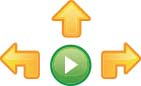
\includegraphics[clip,trim=1.7cm 0cm 1.5cm 1.5cm,width=.3\linewidth]{Arrows.jpg}
\end{center}

Explain how to go on to level 2 \textit{[fig S2.2]}.
Ask them to suggest what blocks of code are needed.

\fig{fig S2.2}{figS2.2.jpg}{1}

\begin{center}
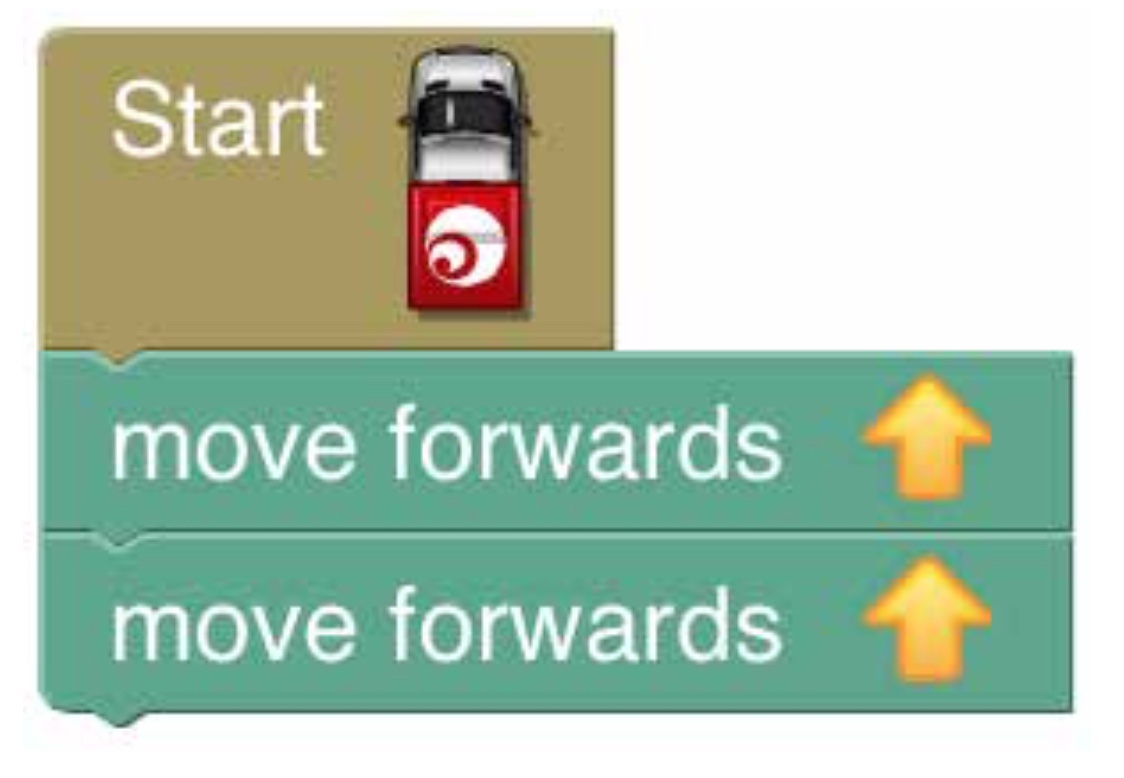
\includegraphics[clip,trim=1.7cm 0cm 1.5cm 1.5cm,width=.667\linewidth]{codeblocks.jpg}
\end{center}

Explain that the blocks of code are the instructions you are giving the computer to make the van move.

\section*{Paired or individual activity}

Give the class a chance to access the app and try levels 1 and 2 themselves.

You will need to have shown the children how to log into the app, using the account details you have created by setting up your class \textit{[fig S2.3]}.

\fig{fig S2.3}{figS2.3.jpg}{1}

Some children will find the Left and Right van cards useful here to help them select the correct code block for their turns.

\section*{Mini review}

Demonstrate level 3 \textit{[fig S2.4]} on the IWB.
\keyquestion{What new command would we need here?}

\fig{fig S2.4}{figS2.4.jpg}{1}


Ask the children to talk to their partner and write on their whiteboards what instructions they need to drive the van to the house.

Ask a volunteer to test their solution on the IWB.
\keyquestion{Can you read out your code?}

Key question: \keyquestion{If we changed the order of the instructions, would it matter?} (Test and see).

Make the point that the order of instructions is important.

Add the word \keyword{sequence} to your code word wall.

Demonstrate level 4 \textit{[fig S2.5]} on the IWB.
\keyquestion{What new command would we need here?}

\fig{fig S2.5}{figS2.5.jpg}{1}

\section*{Paired activity}

Ask the children to continue working up to level 4.

\section*{Share and review}

Look at level 5 \textit{[fig S2.6]} together on the IWB and give the children the printed sheets to match.
Assess children's learning by asking them to predict the code needed for this more interesting road on their whiteboards, or by sequencing the KS1 Blockly cards.

\fig{fig S2.5}{figS2.6.jpg}{1}

\keyquestion{Can you predict the sequence of code for this route?}

Explain that next time you are going to look at longer roads with lots of turns.

Recap on what the world \keyword{algorithm} means and add this display card to your code wall.

(See Glossary).


\end{lessonplan}

\end{document}
